% !TeX root = RJwrapper.tex
\title{\pkg{fitzRoy} - An R Package to Encourage Reproducible Sports Analysis}
\author{by Robert Nguyen, James Day, David Warton and Oscar Lane}

\maketitle

\abstract{
The importance of reproducibility, and the related issue of open access to data, has received a lot of recent attention. Momentum on these issues is gathering in the sports analytics community.  While Australian Rules football (AFL) is the leading commercial sport in Australia, unlike popular international sports, there has been no mechanism for the public to access comprehensive statistics on players and teams. Expert commentary currently relies heavily on data that isn't made readily accessible  and this produces an unnecessary barrier for the development of an inclusive sports analytics community.
We present the R package \pkg{fitzRoy} to provide easy access to AFL statistics.
}


\section{Introduction}

Access to data is the key enabling tool for any sports analytics community. Most major international sports have a mechanism to provide free access to match statistics, for example, \href{https://cran.r-project.org/web/packages/ballr/ballr.pdf}{ballR} for NBA, \href{https://cran.r-project.org/web/packages/Lahman/Lahman.pdf}{Lahman}  for baseball and \href{https://github.com/skoval/deuce}{deuce} for tennis. Access to sports data can be used by fans, clubs and researchers to better predict match outcomes, to inform decisions and better understand the sport. For example \citep{romer2006firms} helped change the way teams evaluate 4th down decisions in the NFL, and the way the NBA is played has changed becoming more three point focused \citep{goldman2013live}. Sports analytics has also proved a popular avenue for modern data journalism for example, \href{https://fivethirtyeight.com}{Fivethirtyeight} is a popular culture website with a strong analytics following, which publishes models daily across a variety of sports. This sort of product can only be constructed given a publicly available source of sports data.



The Australian Football League (AFL) is the national league of Australia's national winter sport, Australian Rules Football. This is the largest commercial support in Australia with over 1 million club members, a 2.5 billion dollar broadcast rights deal and a participation level of 1.649 million. No current AFL statistics website provides easy access to data for a growing analytical fan base. The Australian Football League (AFL) has an official data provider, Champion Data, which is 49\% owned by the AFL. Champion Data have the licence to collect the data for all AFL games and then charge clubs and media organisations fees to access the data. There are two leading websites of publicly available data, \href{https://afltables.com/afl/aflindex.html}{afltables} and \href{https://www.footywire.com}{footywire}, but data are not available in an easy-to-use form. For example, match statistics are listed on separate web pages for different matches, so hours of time would be required to compile data from over 200 different webpages in order to do an analysis across a single season. Hence, unfortunately, there are significant financial and logistical barriers to prospective analysts and fans studying the game, which stagnates progress advancing our understanding of AFL.



This paper describes the \CRANpkg{fitzRoy}  package, the first package to provide free and easy access to data on the AFL, with match and player data for the men's competition\footnote{fitzRoy used to contain access to the AFLW (AFL Womens) data, but unfortunately the data was removed from official AFL media, we are committed to adding AFLW data again, once it comes back}. Web scraping tools have been developed that provide easy, up-to-date access to AFL match and player box statistics across the history of the game, since 1897, using open source data. The package also provides tools to link match and player data to expert tips from popular websites.  For the first time, fans can evaluate the performance of tipsters themselves andcompare them to the betting market.


\section{What is \pkg{fitzRoy}?}

We developed \pkg{fitzRoy}, an R package  that allows users to access Australian Rules Football statistics from various websites easily with R.
The \pkg{fitzRoy} package allows users access to popular AFL statistics websites such as \href{https://afltables.com/afl/afl_index.html}{afltables} and \href{https://www.footywire.com}{footywire}. These are the two most widely used data repositories in the AFL, which have existed since the late 1990s, and while they are not official repositories, the AFL has not tried to take them offline. However, the data on these websites is not available in an easy-to-use form, e.g. match statistics are stored across different web pages for each match, so compiling season statistics would involve harvesting data from hundreds of webpages. The \pkg{fitzRoy} package compiles match or player data into a single frame, and also allows users to access popular bloggers' AFL models via the \href{https://squiggle.com.au}{squiggle} website.


A popular website called \href{https://afltables.com/afl/seas/2018.html}{afltables}  contains AFL-VFL match, player and coaching stats, records and lists from 1897\footnote{The first year of VFL}. The website \href{https://afltables.com/afl/afl_index.html}{afltables} has been used in research for topics such as umpire racism \citep{lenten2017racial}, umpires assessment of players \citep{lenten2019sentiment}, modelling of the AFL game \citep{kiley2016game}, fixture difficulty \citep{lenor2016rivalry} and drafting \citep{lenten2018evaluating}. The umpire studies would not have been possible with \href{https://www.footywire.com}{footywire} data as umpire information isn't contained on the game pages.

The \href{https://www.footywire.com}{footywire} website has data back to 1965, but while it does not have as many seasons of data, it has additional game variables not included in \href{https://afltables.com/afl/afl_index.html}{afltables}. One example is Super Coach score, sometimes used as a proxy for player value \citep{marshall2017effect}. Other examples of variables contained within footywire are tackles inside 50, intercepts and marks inside 50 to name a few.

\href{https://squiggle.com.au}{Squiggle} is a unique website in the AFL sporting landscape. It contains game analyses but it also aggregates popular AFL bloggers' tips each week. From \href{https://squiggle.com.au}{squiggle} users are able to get each models probability of win, margin prediction and a leaderboard based on \href{http://probabilistic-footy.monash.edu/~footy/about.shtml#info}{bits} which has been made popular by the Monash probability footy tipping competition\footnote{http://probabilistic-footy.monash.edu/~footy/}.


\section{Building \pkg{fitzRoy}}

The name \pkg{fitzRoy} comes from  the Old Fitzroy hotel in Sydney where the idea for the package was first conceived. It is also the name of one of the foundation clubs of the Australian Football League, which since merged with another club, and is now called the Brisbane Lions.

We used the R packages \CRANpkg{Rvest} \citep{Rvest}, \CRANpkg{dplyr} \citep{dplyr}, \CRANpkg{purrr} \citep{purrr} and \CRANpkg{XML} \citep{xml} to construct our web-scraper functions that collate data from \href{https://afltables.com/afl/afl_index.html}{afltables} or \href{https://www.footywire.com}{footywire} into a single data frame. These websites update immediately on completion of each round, hence so does data accessed via \pkg{fitzRoy} scraper functions. The key functions accessing \href{https://afltables.com/afl/afl_index.html}{afltables} player and match statistics are \code{get\_afltables\_stats} and \code{get\_afl\_match\_data}, respectively, and \href{https://www.footywire.com}{footywire} data are accessed via the \code{get\_footywire\_stats} function. These functions form the backbone of the package.

\begin{figure}
\centerline{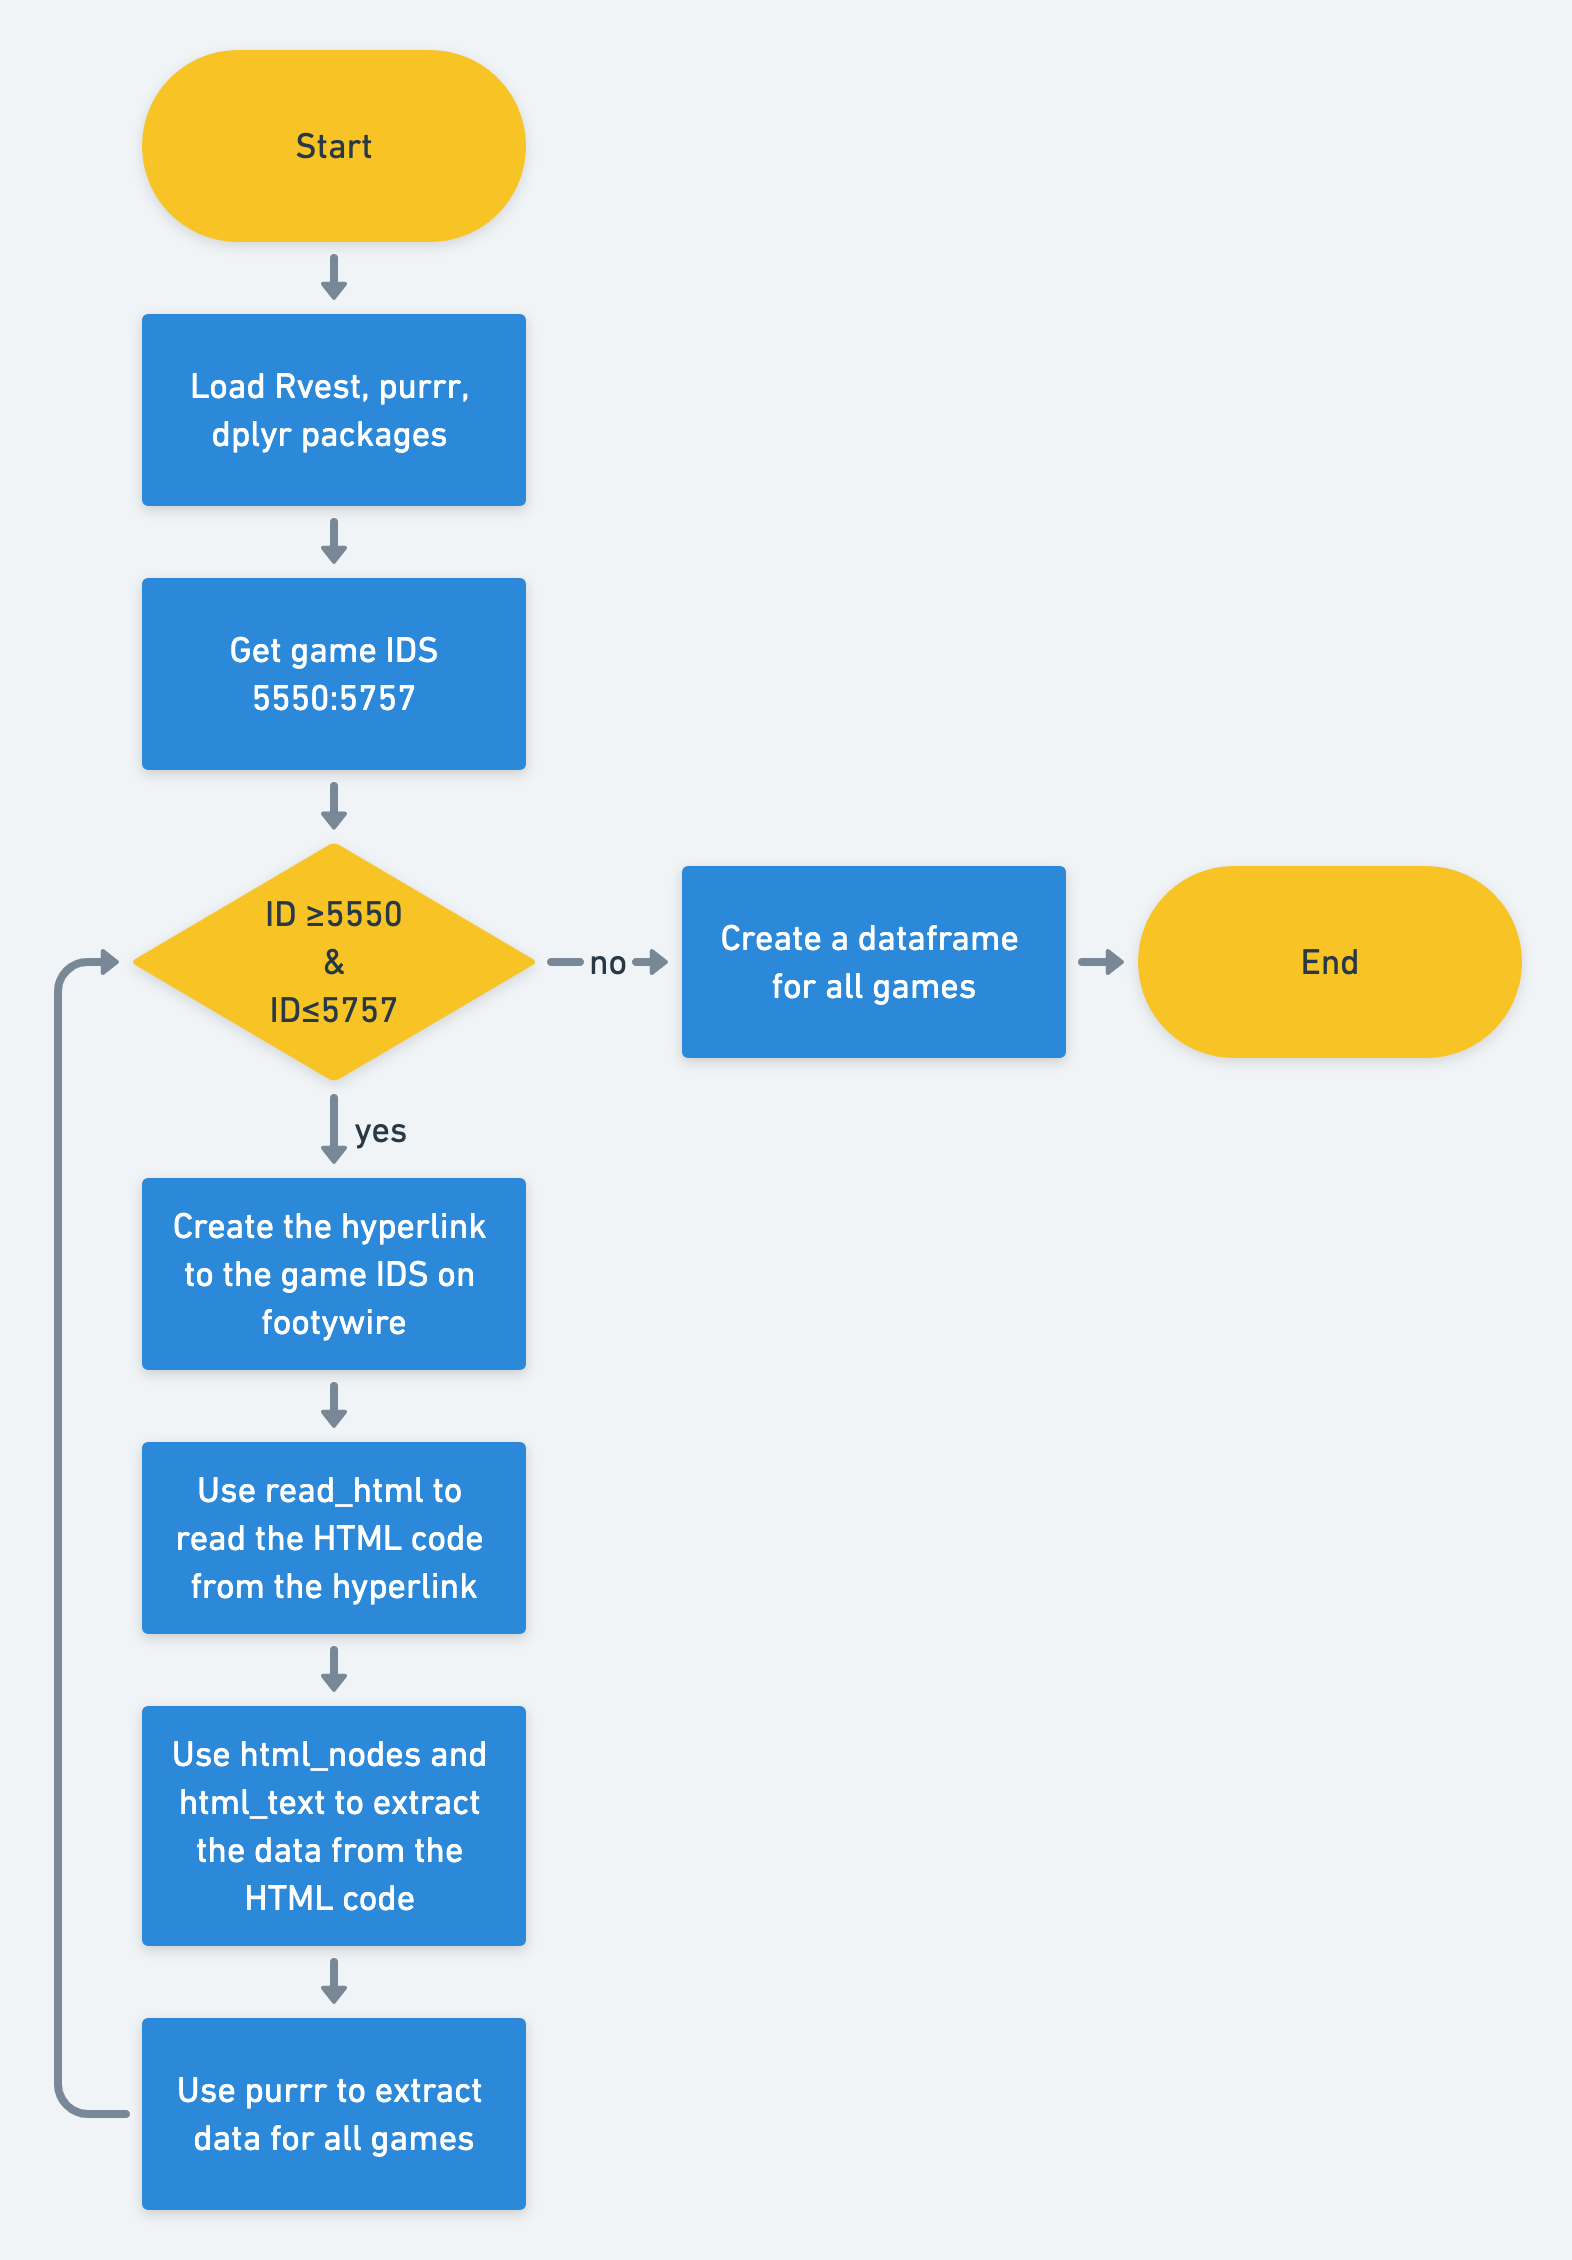
\includegraphics[scale=0.25]{webscrapR.png}}
\caption{Work flow for \pkg{fitzRoy} web-scrapers game IDS 5550 to 5757 refer to the 2013 AFLM Season.}
\end{figure}



\section{Applications of \pkg{fitzRoy}}


\subsubsection{Match Data (Scores)}

The \code{get\_match\_results} function can be used to obtain match data for any season(s) or team(s). For example to get the game scores for Fitzroy's last AFL season as follows.\footnote{fans of Fitzroy Lions might want to avoid this as it only contains one win (Round 8 vs Fremantle Dockers)}

%\begin{lstlisting}[language=R]
\begin{example}
library(fitzRoy)
library(tidyverse)
library(lubridate)
fitzRoy::get_match_results()%>%
mutate(Season=lubridate::year(Date))%>%
filter(Season==1996)%>%
filter(Home.Team=="Fitzroy" | Away.Team=="Fitzroy")
\end{example}
%\end{lstlisting}


\subsubsection{Match Data (Players)}

Fans of Australian Football like many major sports like to keep up to date with leaders of statistical categories. One statistic often of interest is goals scored. Users can come up with the leading goalkicker list for Fitzroy in 1996 as follows.

%\begin{lstlisting}[language=R]
\begin{example}
library(fitzRoy)
library(tidyverse)
fitzRoy::get_afltables_stats(start_date="1996-01-01",
end_date="1997-01-01")%>%
filter(Playing.for=="Fitzroy")%>%
group_by(ID, First.name, Surname)%>%
summarise(Total_Goals=sum(Goals))%>%
arrange(desc(Total_Goals))
\end{example}
%\end{lstlisting}

 We can see that  Anthony  Mellington won the goalkicking award for Fitzroy with a modest total of 22 goals for the 1996 season. 


\subsection{Building Sports Models}

Sports models are commonly derived using an Elo system which only needs scores \citep{ryall2010optimized}.
The \pkg{fitzRoy} package readily provides a data frame of match scores, from which it is straightforward to construct an Elo to predict future match outcomes, as below.

%\begin{lstlisting}[language=R]
\begin{example}
library(fitzRoy)
library(tidyverse)
library(elo)
library(lubridate)

# Get data
results <- fitzRoy::get_match_results()
results <- results %>%
mutate(seas_rnd = paste0(Season, ".", Round.Number),
First.Game = ifelse(Round.Number == 1, TRUE, FALSE)
)

fixture <- fitzRoy::get_fixture()
fixture <- fixture %>%
filter(Date > max(results$Date)) %>%
mutate(Date = ymd(format(Date, "%Y-%m-%d"))) %>%
rename(Round.Number = Round)

# Simple ELO
# Set parameters (these should be optimised!)
HGA <- 30
carryOver <- 0.5
B <- 0.03
k_val <- 20

# Create margin function to ensure result is between 0 and 1
map_margin_to_outcome <- function(margin, B) {
1 / (1 + (exp(-B * margin)))
}

# Run ELO
elo.data <- elo.run(
map_margin_to_outcome(Home.Points - Away.Points, B = B) ~
adjust(Home.Team, HGA) +
Away.Team +
group(seas_rnd) +
regress(First.Game, 1500, carryOver),
k = k_val,
data = results
)

as.data.frame(elo.data)
as.matrix(elo.data)
final.elos(elo.data)

# Do predictions
fixture <- fixture %>%
mutate(Prob = predict(elo.data, newdata = fixture))

head(fixture)
\end{example}
%\end{lstlisting}



\subsection{Building Player Models}

Box-score statistics, summary statistics of the involvement of each player in each match, contain a rich history of information. Box score statistics led, for example, to the concept of Value Over Replacement Player (VORP) \citep{woolner2001introduction}\footnote{https://www.theringer.com/mlb/2018/2/20/17030428/sherri-nichols-baseball-sabermetric-movement}. Fantasy teams have gained a lot of interest in recent years, and fantasy scores for players tend to be constructed from box-score statistics.

The AFL runs a fantasy sport competition, and \pkg{fitzRoy} could be used to recreate its fantasy points formula, since it is a linear function of box-score statistics.

Box-score AFL data are made readily accessible through \pkg{fitzRoy} using the \code{player\_stats} function.

%\begin{lstlisting}[language=R]
\begin{example}

library(fitzRoy)
library(tidyverse)

df<-fitzRoy::get_footywire_stats(9721:9927)

eq1<-lm(AF ~ K + HB + M + `T` + FF + FA + HO + G + B, data=df)
summary(eq1)
\end{example}
%\end{lstlisting}

While this might seem like a trivial application, footywire only has fantasy scores going back to 2007, however the statistics used for fantasy go all the way back to 1965, with Tackles being first recorded in 1987.

%\begin{lstlisting}[language=R]
\begin{example}

cbPalette <- c("#999999", "#E69F00", "#56B4E9", "#009E73",
"#F0E442", "#0072B2", "#D55E00", "#CC79A7")

fitzRoy::get_afltables_stats(start_date = "1897-01-01",
end_date = "2018-10-10")%>%

group_by(Season)%>%
summarise(
meankicks=mean(Kicks),
meanmarks=mean(Marks),
meantackles=mean(Tackles),
meanfreesfor=mean(Frees.For),
meansfreesagainst=mean(Frees.Against),
meanhitouts=mean(Hit.Outs),
meangoals=mean(Goals),
meanbehinds=mean(Behinds))%>%
gather("variable", "value",-Season) %>%
ggplot(aes(x=Season, y=value, group=variable, colour=variable))+
geom_line()+
scale_colour_manual(values=cbPalette)
\end{example}
%\end{lstlisting}

\begin{figure}
	\centerline{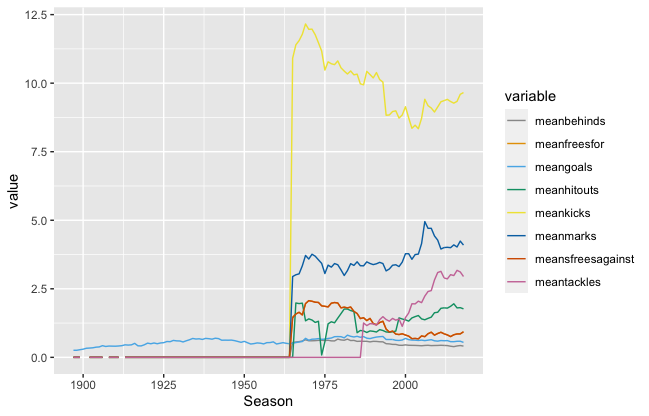
\includegraphics[scale=0.6]{Rplot01.png}}
	\caption{Line graph of mean values of AFLM statistics - By seeing when the line jumps from zero is a quick way to see when a statistic was first collected.}
\end{figure}



Goals have been recorded at a player level throughout the history of the game, and the most recent variable that is used in fantasy (tackles) started being recorded in 1987.

The box-score also contains time on ground so users are readily able to compute points per minute which has been a leading indicator for 2 time winner of fantasy sports  Moreira Magic.\footnote{https://player.whooshkaa.com/shows/chilling-with-charlie}

Champion Data publish Super Coach scores, valued by clubs to inform recruitment decisions and fantasy sport competitions. However the formula for Super Coach scores is propriety and not in the public domain. Following the release of \href{https://github.com/jimmyday12/fitzRoy}{fitzRoy}, one well-known blogger attempted to re-create it with a linear model, and managed an R-squared of 91.6\footnote{http://www.matterofstats.com/mafl-stats-journal/2018/10/7/a-first-attempt-at-combining-afl-team-and-player-data-in-a-predictive-model}\footnote{This is impressive as Champion data uses data not available within \pkg{fitzRoy} and its weighted by time and game margin.}

%\newpage

\subsection{Able to Compare Popular Models}

Blogging has taken off around the world with popular websites such as \href{https://fansided.com}{fansided}, \href{http://fivethirtyeight.com}{fivethirtyeight} and \href{https://www.theringer.com}{the ringer} proving popular among the overseas sporting community.
To help promote other people who do modeling work and make their work available online, we provide access to squiggle, the most popular aggregator website in the AFL. This means that the behaviour of different tipsters' models can be analysed easily.

%\begin{lstlisting}[language=R]
\begin{example}

library(fitzRoy)
fitzRoy::get_squiggle_data("tips")
\end{example}
%\end{lstlisting}

The above command will enable a user to get the tips from popular blogging sites such as \href{https://squiggle.com.au}{squiggle}, \href{http://www.matterofstats.com}{matterofstats} and \href{https://www.liveladders.com/AFL/}{liveladders} among many. This means that different tipsters models behaviours can be analysed easily. For example studying how they take into account home ground advantages.


\section{Future Developments}

The developers of \pkg{fitzRoy} is committed to giving users the data to analyse the game. In the future this means updating the Womens AFLW data once it becomes available online, updating the scrapers to include the AFL website.

\section{Summary}



The \pkg{fitzRoy} package offers a springboard for sports analytics in the AFL community. It provides easy access to publicly available AFL data, and we have illustrated how this can be used to predict match outcomes and to rank players. In future work we plan to build a statistical model for AFL match outcomes and its key predictors, along the lines of \citep{yurko2018nflwar,deshpande2016estimating}. There are endless possibilities: clubs might use it to inform on player recruitment \citep{on2010value} and team style \citep{greenham2017pilot}; researchers and enthusiasts can use it to better understand the game; there are obvious betting implications \citep{bailey2000identifying}; and educators can use it as a teaching tool.

The \pkg{fitzRoy} package was only released in 2018 but has already been used by AFL club analysts and bloggers who are now able to access data and develop content they weren't previously able to do (\emph{e.g.}\ \href{http://www.matterofstats.com/mafl-stats-journal/2019/1/5/estimating-afl-player-value}{VORP}). The AFL analytics community is develops rapidly, and it is exciting to see where it will go over the coming seasons.



\bibliography{nguyen-warton-day.bib}



\address{Robert N. Nguyen\\
  School of Mathematics and Statistics\\
  University of New South Wales\\
  Sydney,NSW 2052 Australia\\
  \email{robert.nguyen@unsw.edu.au}}

\address{James T. Day\\
	Fusion Sport\\
   Australia\\
	\email{jamesthomasday@gmail.com}}

\address{David I. Warton\\
  School of Mathematics and Statistics and\\
  Evolution \& Ecology Research Centre\\
University of New South Wales\\
Sydney,NSW 2052 Australia\\
  \email{David.Warton@unsw.edu.au}}

\address{Oscar Lane\\
\email{lane.oscar@gmail.com}}
